\documentclass[tikz,border=2mm]{standalone}

\usetikzlibrary{arrows.meta,chains,shapes.symbols}

\begin{document}

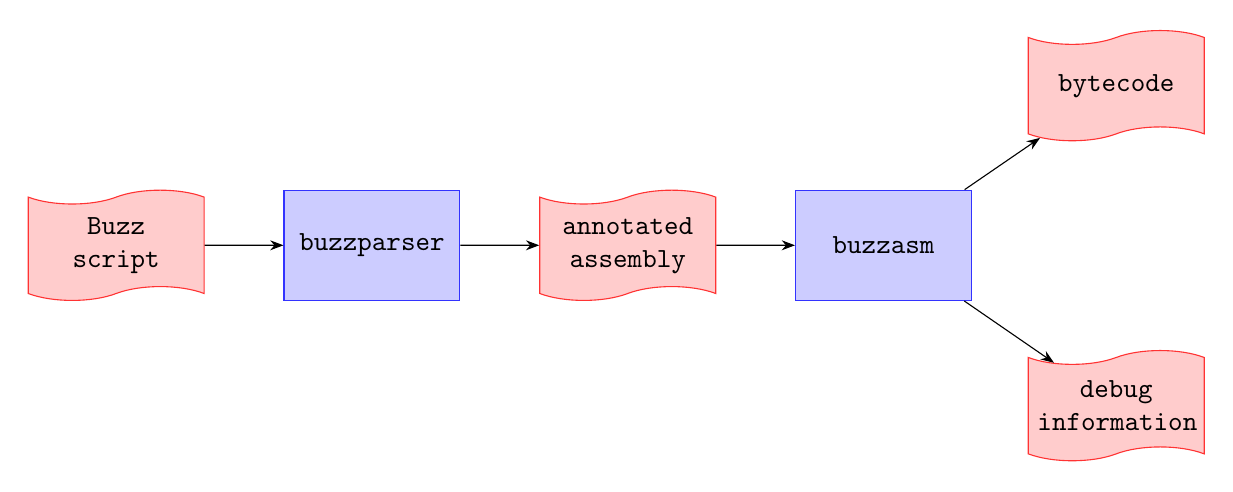
\begin{tikzpicture}[
  start chain,
  node distance=1cm,
  every node/.style={draw,on chain,join,minimum size=1.4cm,text width=2cm,align=center,font=\tt},
  every join/.style={-Stealth},
  output/.style={tape,draw=red!80,fill=red!20},
  process/.style={rectangle,draw=blue!80,fill=blue!20}]
  
  \node(script)   [output] {Buzz\\script};
  \node(parser)   [process]{buzzparser};
  \node(asm)      [output] {annotated\\assembly};
  \node(assembler)[process]{buzzasm};
  
  \begin{scope}[start branch=up going {above right}]
    \node(bytecode)[output]{bytecode};
  \end{scope}
  \begin{scope}[start branch=down going {below right}]
    \node(debug)   [output]{debug\\information};
  \end{scope}

\end{tikzpicture}

\end{document}